\section{Approach} \label{sec_approach}

\begin{figure}[t]
\centering
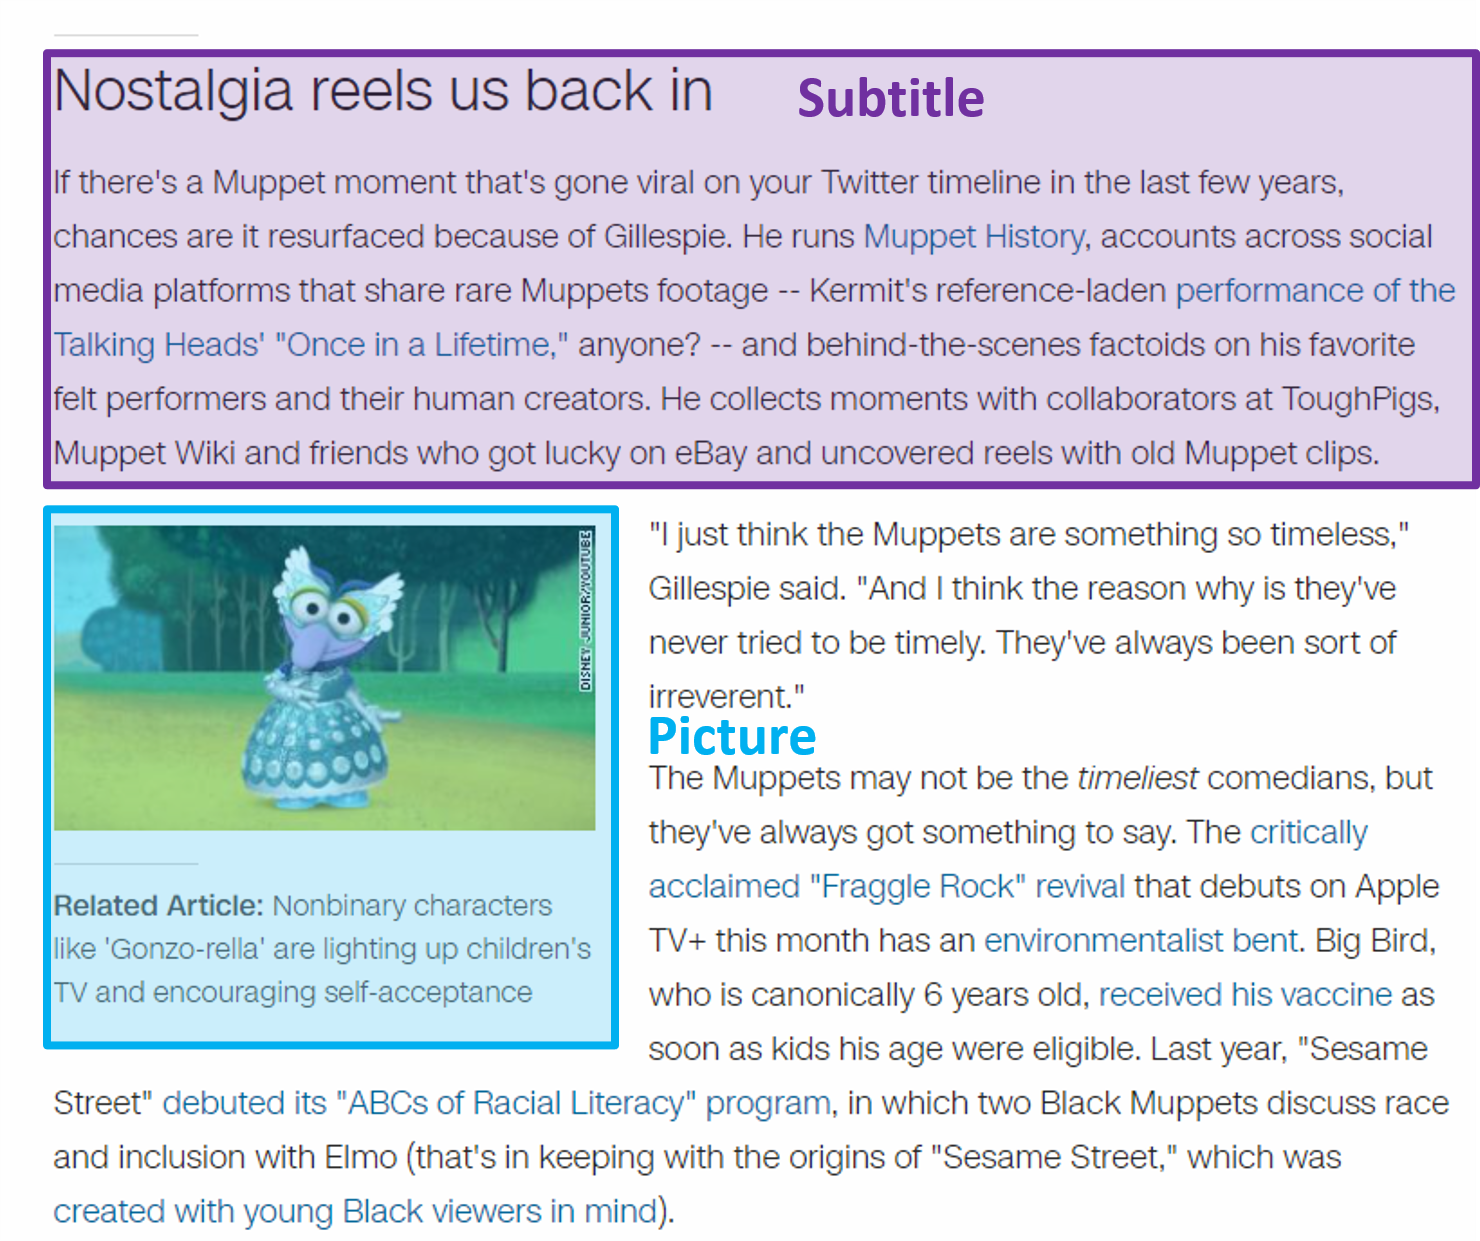
\includegraphics[width=1\columnwidth]{vis_example2}
\caption{The main content part of a sample article with subtitle (purple shading) and picture (blue shading)}
\label{vis_example2}
\end{figure}

This section introduces our approach to rank hyperlinks, which mainly takes two steps. The first step is to extract hypertext link features from the web pages. For the next step, we feed these features into the Learning to Ranking algorithm to obtain the prediction result.

\subsection{Learning to Rank}

Learning to Rank (L2R) is a supervised machine learning technique that aims to produce a ranking function $F$ with the set of feature vectors $\vec{x}$ to approximate the ground-truth rankings $y$. L2R is trained by optimizing the loss function $L(F(\vec{x_j}), y_j)$ for all items $1 \leq j \leq n$, which reflects the deviation of the predicted rankings from the ground-truth rankings. 

According to different realizations of the loss function, L2R algorithms can be classified into 3 groups: pointwise, pairwise and listwise \cite{liu2011learning}. Listwise L2R algorithms like LambdaMart \cite{wu2010adapting} have shown competitive performance in many ranking tasks for their holistic utilization of the ranking list. Therefore, we choose LambdaMart as our ranking algorithm. 

\subsection{Visual Features} \label{sec_vis_feature}

How frequently a hyperlink gets clicked highly depends on its visual position. Some regions are more exposed to the readers and can thus obtain more attention. To characterize the effect of visual feature on the click popularity of hyperlinks, we propose five visual features for hyperlink ranking: \emph{section position}, \emph{distance to the nearest picture}, \emph{distance to the nearest subtitle}, \emph{distance to nearest table} and \emph{within table}. All the visual features we have proposed do not require rendering. Instead, we extract components like pictures and tables with regular expressions.

\subsubsection{Section Position}

In \cite{lamprecht2017structure}, the authors found that a large share of user clicks are from links in the first several sections. We can exploit this finding as one of the features. Figure \ref{vis_example1} shows the beginning part of a sample article. In Figure \ref{vis_example1}, the lead section has been highlighted. When browsing this web page, we tend to focus more on the first several sections. For example, in the lead section, the hyperlink named \emph{alledged leaks} usually gets more clicks. In the rest sections, many hyperlinks remain unspotted until readers scroll down the web page. 

Given this finding, we propose a feature named \emph{section position} to represent which section the hyperlink is located in. The feature takes value of $x$ if the hyperlink is placed within the $x$th section. 

\subsubsection{Subtitle}

Subtitles are usually presented with big fonts or bold texts. The subtitle part is highlighted in Figure \ref{vis_example2}. When the readers start reading the section under the subtitle, these hyperlinks near the subtitles like \emph{Muppet History} are easier to be noticed. To characterize the effect of subtitles on hyperlink click popularity, we propose \emph{distance to the nearest subtitle} as one of the visual features.

\subsubsection{Picture}

Pictures are always eye-catching. When browsing web pages, readers tend to pay more attention to the pictures. Some links placed near to the picture are more likely to get clicked. For example in Figure \ref{vis_example2}, the hyperlink \emph{critically acclaimed "Fraggle Rock" revival} is placed near to a picture. We use \emph{distance to the nearest picture} as a feature to indicate whether the hyperlink is placed somewhere near to a picture.
    
\subsubsection{Table}

Apart from pictures and titles, tables can also be attractive. In Figure \ref{vis_example3}, the hyperlink \emph{Apocalypto} is placed quite near to the table, which is likely to get more clicks. We define the distance between the hyperlink and its nearest table as a feature called \emph{distance to the nearest table}.

Assuming that whether a link is positioned within a table affects how frequently the hyperlink will get clicked, we propose \emph{within table} as another feature, which could help in predicting the click popularity of hyperlinks. If the link is placed within the table, the feature would take the value of 1, and 0 otherwise.

\begin{figure}[t]
\centering
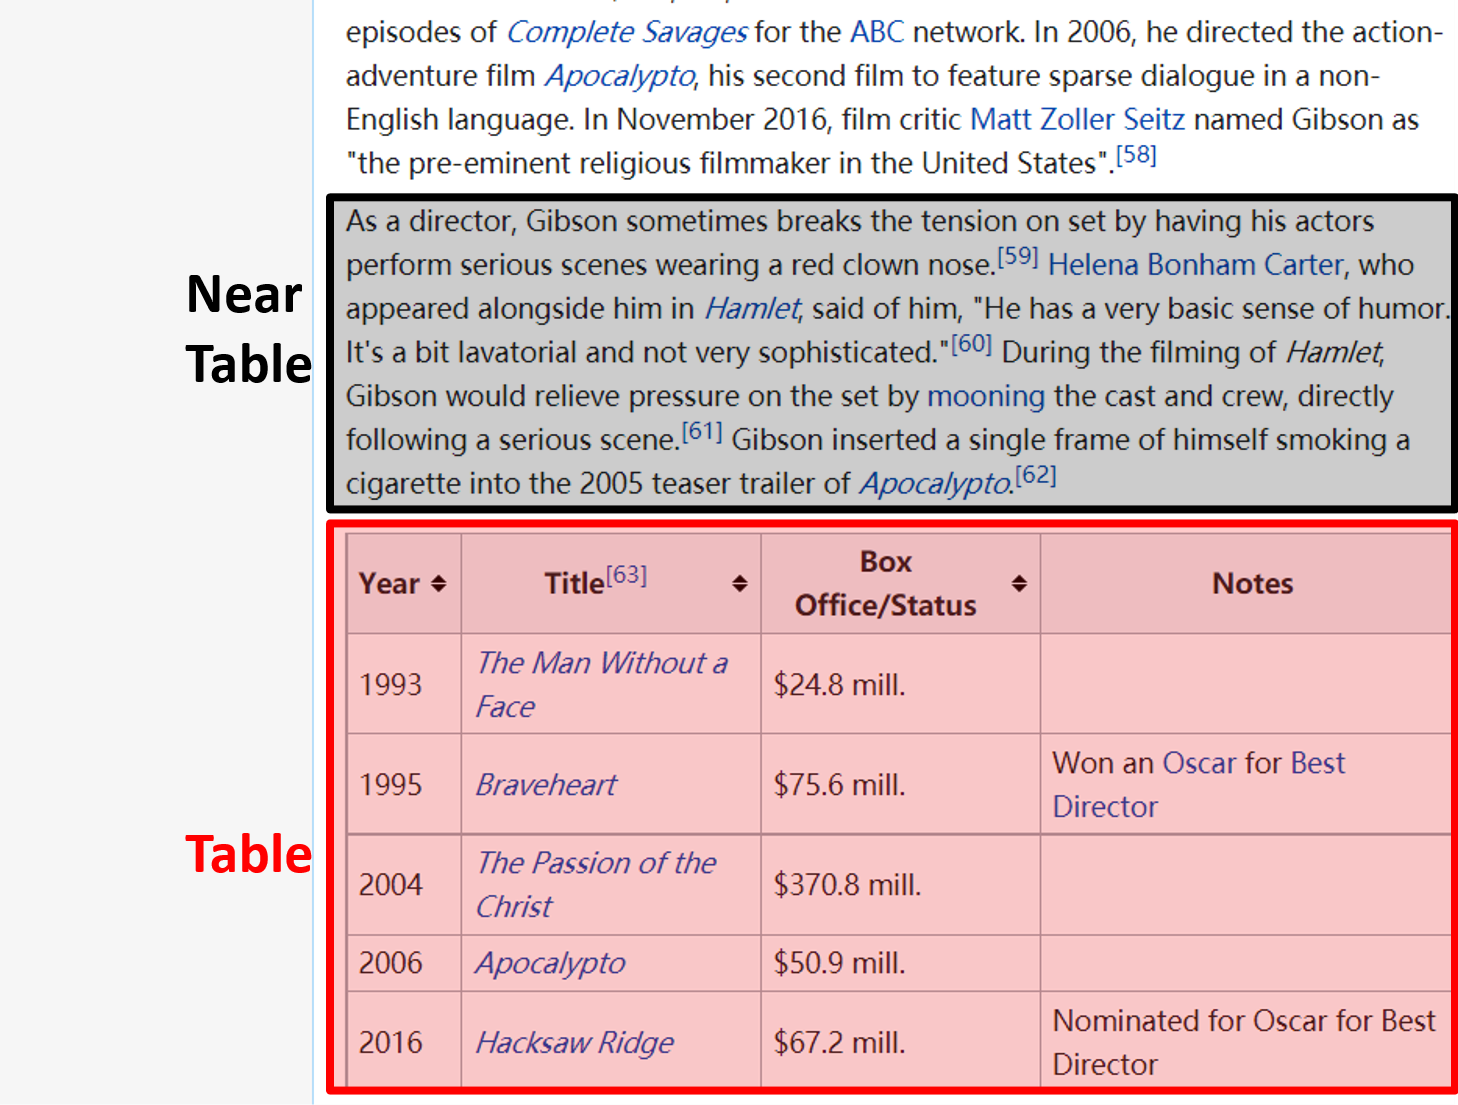
\includegraphics[width=1\columnwidth]{vis_example3}
\caption{The main content part of a sample article with near table section (black shading) and table (red shading)}
\label{vis_example3}
\end{figure}